% Chapter 1

\chapter{\color{thesisBlue} High Dimensional Stimulus spaces for neural data} % Main chapter title

\label{ch:optim} % For referencing the chapter elsewhere, use \ref{Chapter1} 

%----------------------------------------------------------------------------------------

% Define some commands to keep the formatting separated from the content 
\newcommand{\keyword}[1]{\textbf{#1}}


%----------------------------------------------------------------------------------------
%	Chapter intro
%----------------------------------------------------------------------------------------
In this section I will introduce various analysis approaches for quantifying neural population tuning to stimulus spaces of arbitrary dimensionality. These approaches will first be applied to a simulated population of neurons in order to build intuition for the neural data in chapter \ref{ch:maps}.


%----------------------------------------------------------------------------------------
%	3D NEURON SIMULATION SECTION
%----------------------------------------------------------------------------------------


\section*{\color{sectionBlue} Simulated Neural Population}
I begin by referring back to the 1D tuning curve from chapter \ref{ch:intro}, figure \ref{fig:tuningIntro}. I use the simple gaussian tuning curve as a template, and apply it to a small population of 3 neurons along 3 arbitrary stimulus dimensions. The choice of 3D neural state space and 3D stimulus space comes from the curse of dimensionality; in order to completely sample the spaces, 3 dimensions is the maximum due to combinatorics. For the sake of simplicity I will begin with a set of axioms with which to constrain my artificial neurons:

\begin{enumerate}
	\item \label{ax:bounds} Neurons have a minimum ($0$) and maximum ($R_{max}$) firing rate 
	\item \label{ax:gauss} Neurons are gaussian tuned to each stimulus dimension.
	\item There is one global maximum stimulus per neuron, which lies at a point in the stimulus space ($\harpoon{\rho_n}$).
	\item \label{ax:distfx} Neurons' responses to stimuli is some function of distance between its' preference and the stimuli
	\item Tuning to each stimulus dimension is independent of other dimensions (e.g. color and orientation tuning are assumed independent).
	\item \label{ax:nocorr} Neurons' responses to stimuli are independent from other neurons
\end{enumerate}

Later on, I will reduce the number of assumptions by adding in neural correlations and tuning dependence, but for now start with the simplest model. 

\subsection*{Defining the Population Response Function}

Due to axiom \ref{ax:nocorr}, I can calculate the responses of each neuron independently and define a single response function $f_n(\harpoon\theta)$. This function is bounded by $f_n(\harpoon\theta) \in [0, R_{max}]$ according to axiom \ref{ax:bounds}. If we combine axioms \ref{ax:gauss} and \ref{ax:distfx} with these natural boundaries, we get equation \ref{eq:response}, which defines the neural response in terms of the stimulus parameters ($\harpoon\theta$), peak firing rate ($R_{max}$), and decay term ($D_n(\harpoon\theta)$) for a stimulus space of arbitrary dimensionality.

\begin{equation}
	\label{eq:response}
	f_n(\harpoon{\theta}) = R_{max} \cdot e^{D_n(\harpoon\theta)}
\end{equation}

The decay term, ${D_n(\harpoon\theta)} \in [-\infty, 0]$, depends on both the euclidean distance between $\harpoon\theta$ and $\harpoon{\rho_n}$, and the neurons' tuning matrix ($\tau_n$). $\tau_n$ determines the rate at which the firing rate decays as $\harpoon\theta$ diverges from $\harpoon{\rho_n}$.

\begin{equation}
	\label{eq:decay}
	D_n(\harpoon\theta) = (\harpoon{\rho_n} -\harpoon\theta)^\top \cdot \tau_n \cdot (\harpoon\theta-\harpoon{\rho_n})
\end{equation}

Neurons therefor respond maximally to their preferred stimulus $\harpoon{\rho_n}$ at a rate of $R_{max}$. As the stimulus parameters differ along any dimension, this maximum response decays exponentially at a rate defined by $\tau_n$.

\begin{table}
	\centering
	\begin{tabular}{|c|c|}
		\hline
		\textbf{Symbol}       & \textbf{Description} \\
		\hline
		$\harpoon\theta$      & Vector of stimulus values for presented stimulus \\
		$\harpoon{\rho_n}$    & Vector of preferred stimulus values for neuron $n$ \\
		$f_n(\harpoon\theta)$ & Response in $\frac{spk}{s}$ for neuron $n$ to stimulus $\harpoon\theta$ \\
		$D_n(\harpoon\theta)$ & Decay term for neuron $n$ to stimulus $\harpoon\theta$ \\
		$R_{max}$             & Maximum firing rate \\
		$\tau_n$              & Tuning matrix for neuron $n$ \\
		\hline
	\end{tabular}
	\label{tbl:symbols}
\end{table}


\subsection*{Deterministic Simulations}


\begin{figure}
	\centering
	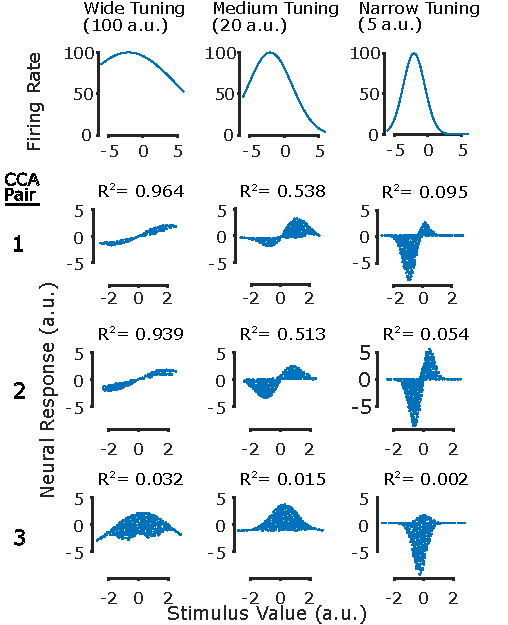
\includegraphics[width=100mm]{tuningWidthSimulationFigure.pdf}
	\caption{The effect of tuning width on CCA.}{This is a great legend that explains so much about stuff...}
\end{figure}


\begin{figure}
	\centering
	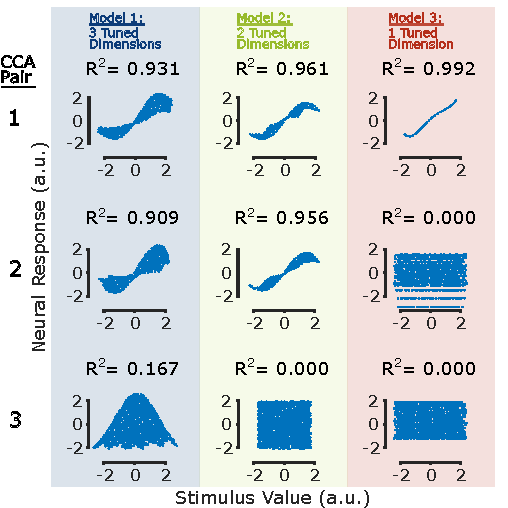
\includegraphics[width=100mm]{invariantDimSimulationFigure.pdf}
	\caption{The effect of untuned stimulus dimensions on CCA.}{This is a great legend that explains so much about stuff...}
\end{figure}


\subsection*{Poisson Variability Simulations}


%----------------------------------------------------------------------------------------
%	OPTIMIZATION SECTION
%----------------------------------------------------------------------------------------
\section*{\color{sectionBlue} Optimization}
Consider here, \textbf{EXAMPLE OF EASILY-UNDERSTANDIBLE OPTIMIZATION PROBLEM}. This example demonstrates that optimization, at the outset, is a simple problem. The complexity comes from large, high-dimensional data sets, and the plethora of approaches available. In this chapter, I will first describe the two main classes of optimization. Second, I will link these concepts to functional properties of neurons, focusing heavily on the visual system. I will then compare multiple algorithms when optimizing simulated neural data. 
\subsection*{What is Optimization?}
In its simplest form, optimization begins with an unknown function of inputs $\vec{x}$:
\begin{equation}
	f(\vec{x}) : \mathbb{R}^{n} \rightarrow \mathbb{R}
\end{equation}
where the output of the function is deterministic of it's inputs $\vec{x}$. The goal of optimization is to then find the set of inputs which minimizes (or maximizes) the output of the function $f(\vec{x})$. \textbf{MORE INTRO TO THIS SECTION BEFORE DERIVATIVES}

\subsection*{Derivative-Based Optimization}
\label{sec:DerivB}
\textbf{MORE INTRO TO THIS SUBSECTION}
We an illustrate this using the simple example of a parabola. 
\begin{figure}
	\centering
	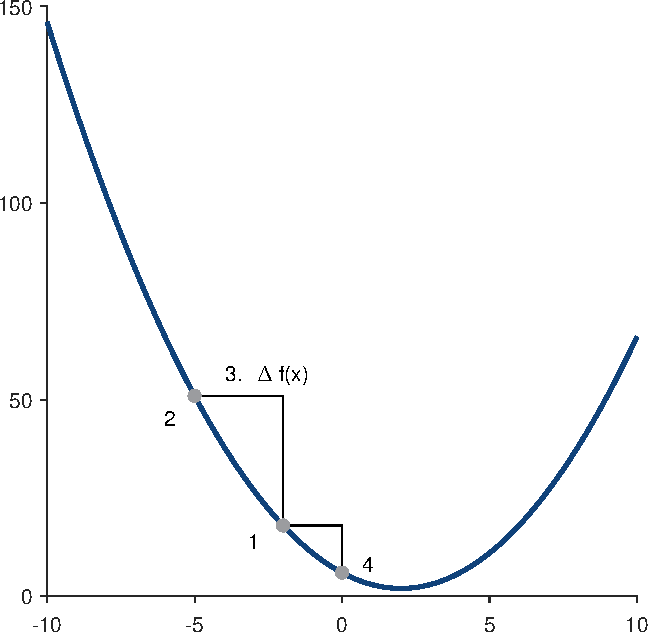
\includegraphics[width=86mm]{parabolaGradient.pdf} 
	\caption{\textit{FigureTitle}}
	\label{fig:parabolaGradient}
\end{figure}
In the realm of low-noise and few variables, optimization is a rather simple problem of calculating the gradient and following it (Figure \ref{fig:parabolaGradient}). In Figure \ref{fig:parabolaGradient}, we test the function by using two random inputs (points 1\&2), calculate the gradient (3), and follow the gradient for the next input (4). This is an iterative process whereby each time we sample the function, we obtain more knowledge about it. Continuing this process will eventually result in $x=2$ as the global minimum. While this may appear obvious, in real world problems the blue line is unknown, necessitating the use of optimization techniques.
Unfortunately, because data is often high-noise and high-dimensional (in the parabola example there is only one input $x$, but most problems have many), calculating gradients quickly becomes computationally intractable in finite time. In addition to these constraints, real-world problems are often non-convex, meaning they have many local minima where gradient descent fails (\textbf{MAYBE NON-CONVEX FIGURE EXAMPLE}). This problem belies standard gradient approaches and lead to the development of Derivative-Free optimization techniques (see \ref{sec:DerivF}).

\subsection*{Derivative-Free Optimization}
\label{sec:DerivF}
\subsection*{Manifold Approximation with Particle Swarm (MAPS)}
\subsection*{Genetic Algorithm}
genetic algorithm doesn't explore the radial dimension well. Even with a-priori knowledge of the proper radius, it doesn't do any better than MAPS because of this (prove it?).

\subsection*{Comparison across algorithms}





%------------------------------------------------------------------------------------


 